\scanpage{43}
suite spectrale de descente\quad spectral sequence of descent\quad VIII 8.1\quad XVII ....
\margin{\handwritten{*}}

Hochschild-Serre (suite spectrale de - )\quad VIII 8.4

\margin{\handwritten{$\mathbb{P}={}$ens. des nbs. premiers\quad $\overline{\underline{\mathrm{IX}}}$ 1.0.}}
\figure{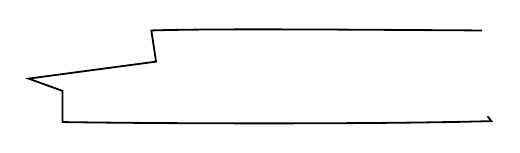
\begin{tikzpicture}[x=.012cm,y=.012cm]
\draw[line width=.65pt] (490,111) .. controls (330,112) and (202,113) .. (140,111) -- (145,78) -- (10,60) -- (46,47) -- (46,14) .. controls (184,12) and (392,12) .. (500,15) -- (496,20);
\end{tikzpicture}}

\unsure{\deleted{F}f|\deleted{f}F}aisceau de p-torsion, \inserted{faisceau de torsion}\quad p-torsion s\unsure{\deleted{b}h|\deleted{h}b}eaf, \inserted{torsion sheaf}\quad IX 1.1
\figure{
\begin{tikzpicture}[x=.012cm,y=.012cm]
\draw[line width=.65pt] (0,44) .. controls (-8,22) and (8,20) .. (28,21) .. controls (155,28) and (295,29) .. (377,19) .. controls (388,18) and (389,0) .. (389,-5);
\draw[line width=.65pt] (389,-5) .. controls (393,8) and (400,35) .. (402,48);
\draw[line width=.65pt] (492,47) .. controls (474,28) and (479,25) .. (499,25) .. controls (570,25) and (670,27) .. (696,17) .. controls (710,13) and (710,0) .. (708,-5);
\draw[line width=.65pt] (708,-5) .. controls (723,24) and (756,35) .. (785,51);
\end{tikzpicture}}

faisceau de ind-p-groupes, faisceau de groupes ind-finis\quad sheaf of ind-p-groups, sheaf of ind-finite groups\quad \unsure{\deleted{Y}I|\deleted{V}I|\deleted{I}Y|\deleted{I}V}X 1.5

localement constant (faisceau - )\quad locally constant sheaf\quad IX 2.0

constructible (faisceau d'ensembles, de groupes, de modules - )\quad constructible \deleted{(\unsure{a}} sheaf of sets, groups or modules\deleted{)}\quad IX 2.3

connexe par arcs (schéma - )\quad arcwise connected scheme\quad IX 2.12

Kummer (théorie de - )\quad IX 3.2

$\underline{G}_m\ ,\ (\underline{G}_m)_X\ ,\ \handwritten{\mathbb{\mu}}_n$\quad IX 3.0
\figure{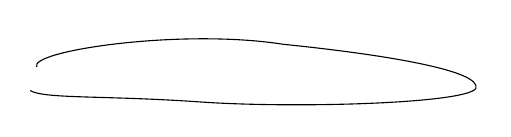
\begin{tikzpicture}[x=.012cm,y=.012cm]
\draw[line width=.4pt] (7,37) .. controls (-2,54) and (160,78) .. (268,61) .. controls (376,50) and (479,33) .. (472,14) .. controls (459,-2) and (278,-7) .. (179,0) .. controls (78,7) and (15,3) .. (0,12);
\end{tikzpicture}}

Hilbert (théorème 90 de - )\quad IX 3.3

diviseur de Cartier\quad Cartier divisor\quad IX 3.4

Artin-\unsure{\deleted{s}S|\deleted{S}s}chreier (théorie de - )\quad IX 3.5

$\handwritten{\wp}$\quad IX 3.5
\figure{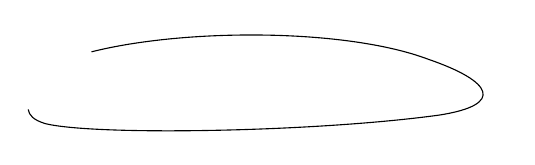
\begin{tikzpicture}[x=.012cm,y=.012cm]
\draw[line width=.4pt] (67,76) .. controls (166,101) and (337,101) .. (424,68) .. controls (491,45) and (506,20) .. (435,9) .. controls (304,-9) and (71,-13) .. (18,0) .. controls (5,4) and (1,9) .. (0,15);
\end{tikzpicture}}

fa\unsure{\deleted{s}i\deleted{i}s|\deleted{i}s\deleted{s}i}ceau gratte-ciel\quad skyscraper sheaf\quad IX 4.1

morphisme trace\quad trace morphism\quad VIII 5.1 , XVII ...
\margin{\handwritten{*}}

$\ell$-dimension cohomologique \inserted{d'un schéma}\quad $\ell$-cohomological dimension \inserted{of a scheme}\quad X 1
\margin{\handwritten{$\ell$}}
\figure{
\begin{tikzpicture}[x=.012cm,y=.012cm]
\draw[line width=.65pt] (307,48) .. controls (292,32) and (303,29) .. (329,27) .. controls (381,25) and (474,22) .. (521,19) .. controls (542,18) and (551,6) .. (551,-4);
\draw[line width=.65pt] (551,-4) .. controls (565,22) and (591,30) .. (612,43);
\draw[line width=.65pt] (858,48) .. controls (845,32) and (850,29) .. (873,28) .. controls (930,26) and (1001,23) .. (1038,16) .. controls (1055,11) and (1065,1) .. (1065,-5);
\draw[line width=.65pt] (1065,-5) .. controls (1089,19) and (1116,29) .. (1140,45);
\end{tikzpicture}}

$\operatorname{cd}_{\unsure{\deleted{l}|\ell}}(X)$\quad X 1

$\operatorname{cdqc}X$\quad X 5.0
\figure{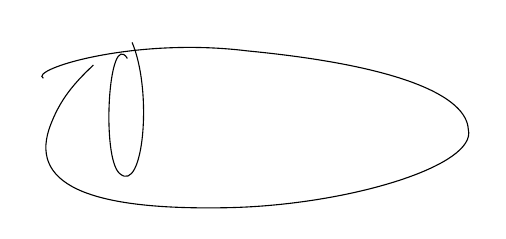
\begin{tikzpicture}[x=.012cm,y=.012cm]
\draw[line width=.4pt] (7,137) .. controls (-9,146) and (102,181) .. (223,166) .. controls (389,150) and (455,117) .. (457,83) .. controls (467,45) and (332,3) .. (204,0) .. controls (64,-3) and (-7,21) .. (13,83) .. controls (24,115) and (41,133) .. (60,151);
\draw[line width=.4pt] (96,158) .. controls (76,190) and (68,52) .. (88,36) .. controls (113,14) and (123,123) .. (101,175);
\end{tikzpicture}}
\margin{\handwritten{$\ell$}}

fibration élémentaire\quad elementary fibration\quad XI 3.1

bon voisin\unsure{\deleted{g}a\deleted{a}g|\deleted{a}g\deleted{g}a}e (relativement à $S$)\quad nice neighbour\unsure{\deleted{g}h|\deleted{h}g}ood relative to $S$\quad \inserted{XI 3.2}
\figure{\begin{tikzpicture}[x=.012cm,y=.012cm]
\draw[line width=.4pt] (9,2) .. controls (-3,27) and (39,68) .. (82,69) .. controls (134,68) and (150,82) .. (162,109) -- (173,82);
\end{tikzpicture}}

théorème de comparaison\quad comparison theorem\quad XI 4.4

$X_{c\deleted{l}}$\quad XI 4.0
\figure{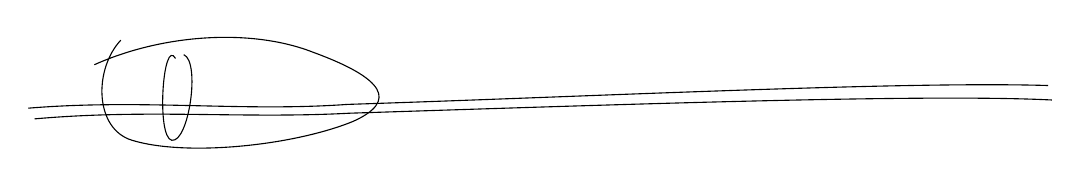
\begin{tikzpicture}[x=.008cm,y=.008cm]
\draw[line width=.4pt] (111,128) .. controls (220,177) and (361,186) .. (458,148) .. controls (573,106) and (593,70) .. (522,38) .. controls (426,-1) and (256,-18) .. (171,8) .. controls (111,26) and (110,121) .. (153,167);
\draw[line width=.4pt] (240,138) .. controls (220,173) and (209,13) .. (234,8) .. controls (261,4) and (280,133) .. (253,144);
\draw[line width=.4pt] (6,59) .. controls (188,74) and (345,53) .. (513,65) .. controls (915,78) and (1396,102) .. (1626,95);
\draw[line width=.4pt] (16,42) .. controls (196,58) and (347,42) .. (516,51) .. controls (951,65) and (1434,82) .. (1632,72);
\end{tikzpicture}}
\margin{\handwritten{Vol. 2}}
\figure{\begin{tikzpicture}\draw[line width=.65pt] (0,0)--(1.2,.95);\end{tikzpicture}}

théorème de changement de base propre\quad proper base change theorem\quad XII 5.1

morphisme de changement de base\quad base change morphism\quad XII 4 , XVII ...
\margin{\handwritten{*}}
% archive sheet number: 42
